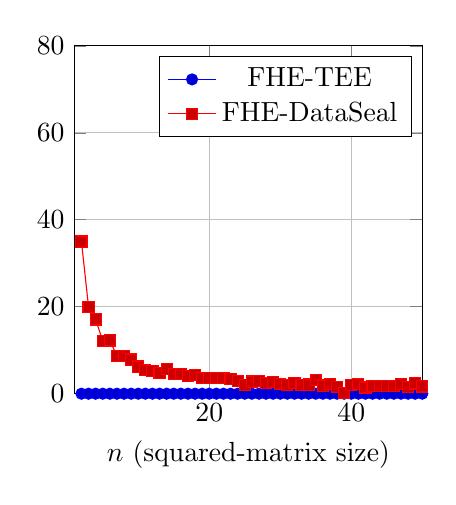
\begin{tikzpicture}
\begin{axis}[
    width=6cm, % Set the width of the plot to the text width of the subfigure
    height=6cm, % You can adjust the height as needed
    xlabel={$n$ (squared-matrix size)},
    legend pos=north east,
    grid=both,
    xmin=1, xmax=50,
    ymin=0, ymax=80
]
\addplot table {
n	FHE-TEE
2	0.00
3	0.00
4	0.00
5	0.00
6	0.00
7	0.00
8	0.00
9	0.00
10	0.00
11	0.00
12	0.00
13	0.00
14	0.00
15	0.00
16	0.00
17	0.00
18	0.00
19	0.00
20	0.00
21	0.00
22	0.00
23	0.00
24	0.00
25	0.00
26	0.00
27	0.00
28	0.00
29	0.00
30	0.00
31	0.00
32	0.00
33	0.00
34	0.00
35	0.00
36	0.00
37	0.00
38	0.00
39	0.00
40	0.00
41	0.00
42	0.00
43	0.00
44	0.00
45	0.00
46	0.00
47	0.00
48	0.00
49	0.00
50	0.00
};
\addlegendentry{FHE-TEE}

\addplot table {
n	FHE-DataSeal
2	34.99
3	19.93
4	17.07
5	12.17
6	12.24
7	8.64
8	8.67
9	7.85
10	6.24
11	5.52
12	5.25
13	4.82
14	5.77
15	4.58
16	4.44
17	4.16
18	4.21
19	3.55
20	3.68
21	3.57
22	3.67
23	3.38
24	2.98
25	1.95
26	2.79
27	2.89
28	2.43
29	2.63
30	2.30
31	1.93
32	2.42
33	1.94
34	2.11
35	3.15
36	1.87
37	2.27
38	1.60
39	0.13
40	1.97
41	2.24
42	1.43
43	1.72
44	1.81
45	1.80
46	1.81
47	2.17
48	1.45
49	2.36
50	1.66
};
\addlegendentry{FHE-DataSeal}

\end{axis}
\end{tikzpicture}